\documentclass[a4paper,11pt]{jsarticle}

% 数式
\usepackage{amsmath,amsfonts}
\usepackage{bm}
% 画像
\usepackage[dvipdfmx]{graphicx}
% 枠付き文章
\usepackage{ascmac}
% 位置調整
\usepackage{float}
% ソースコードの表示
\usepackage{listings,jvlisting}
\lstset{
  basicstyle={\ttfamily},
  identifierstyle={\small},
  commentstyle={\smallitshape},
  keywordstyle={\small\bfseries},
  ndkeywordstyle={\small},
  stringstyle={\small\ttfamily},
  frame={tb},
  breaklines=true,
  columns=[l]{fullflexible},
  numbers=left,
  xrightmargin=0zw,
  xleftmargin=3zw,
  numberstyle={\scriptsize},
  stepnumber=1,
  numbersep=1zw,
  lineskip=-0.5ex
}
\renewcommand{\lstlistingname}{ソースコード}


\begin{document}

\title{
  計算機科学実験及演習4	\\   % title
  \large{音響信号処理 レポート1}	% subtitle
}
\author{下田直樹}
\date{提出日: \today}
\maketitle

\tableofcontents
\clearpage

\section{演習2}
まず、連続した「あいうえお」の振幅スペクトルは図\ref{}のよう。
\begin{figure}[H]
  \centering
  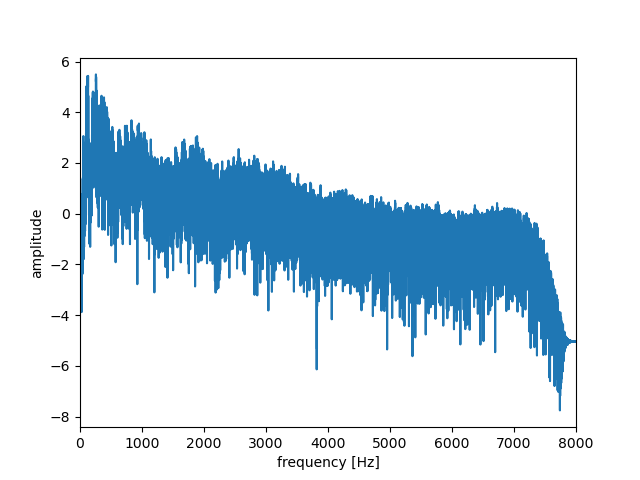
\includegraphics[scale=0.5]{../ex02/img/plot-spectrum-whole_all.png}
  \caption{「あいうえお」の振幅スペクトル}
  \label{spectrum_all}
\end{figure}

また、各音の振幅スペクトルは次のよう。
\begin{figure}[H]
  \centering
  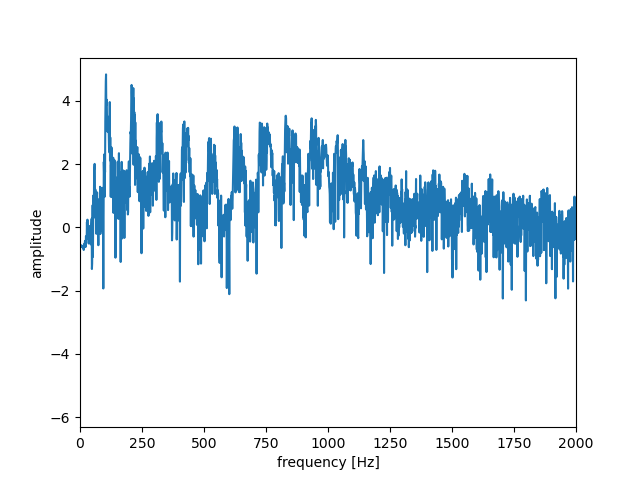
\includegraphics[scale=0.5]{../ex02/img/plot-spectrum-2000_a.png}
  \caption{"あ"の振幅スペクトル}
  \label{spectrum_a}
\end{figure}

\begin{figure}[H]
  \centering
  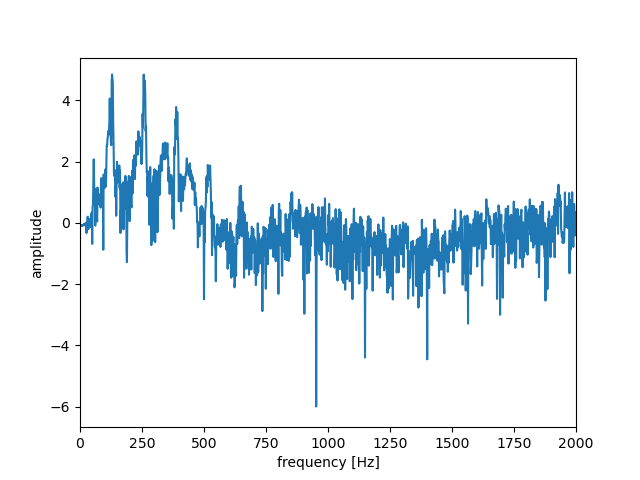
\includegraphics[scale=0.5]{../ex02/img/plot-spectrum-2000_i.png}
  \caption{"い"の振幅スペクトル}
  \label{spectrum_i}
\end{figure}

\begin{figure}[H]
  \centering
  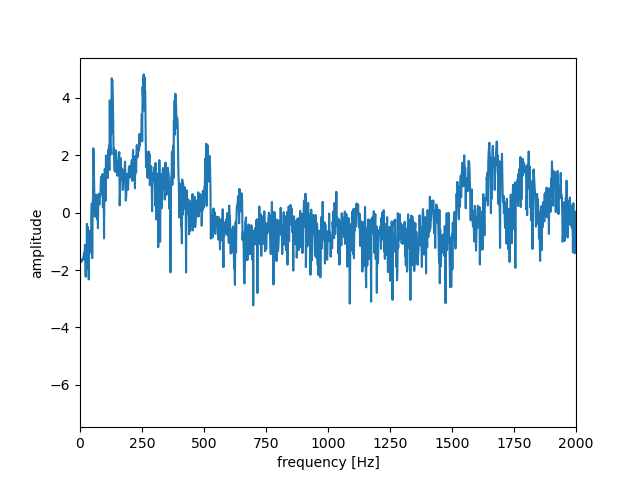
\includegraphics[scale=0.5]{../ex02/img/plot-spectrum-2000_u.png}
  \caption{"う"の振幅スペクトル}
  \label{spectrum_u}
\end{figure}

\begin{figure}[H]
  \centering
  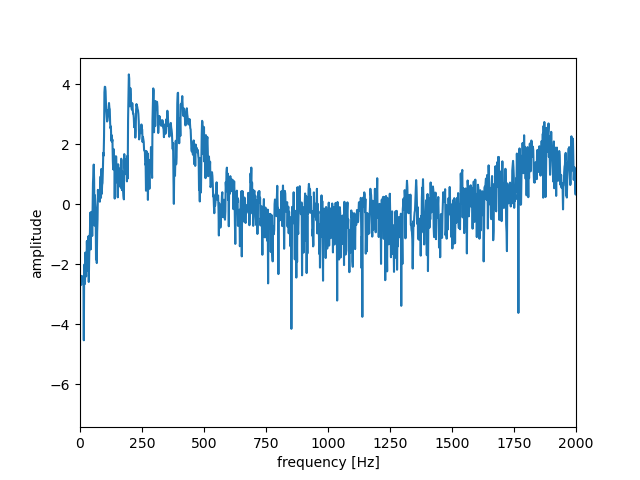
\includegraphics[scale=0.5]{../ex02/img/plot-spectrum-2000_e.png}
  \caption{"え"の振幅スペクトル}
  \label{spectrum_e}
\end{figure}

\begin{figure}[H]
  \centering
  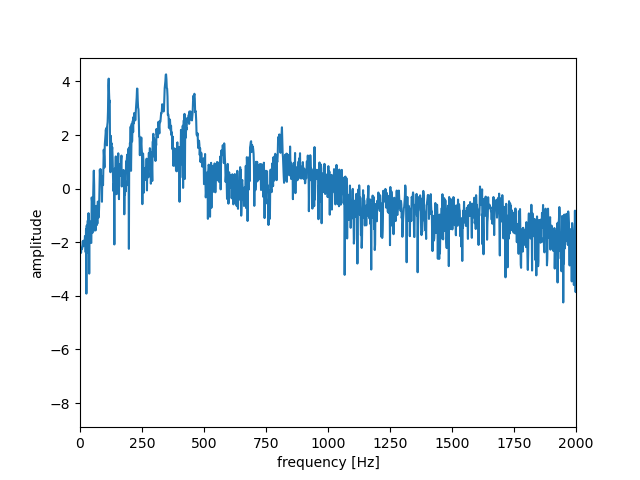
\includegraphics[scale=0.5]{../ex02/img/plot-spectrum-2000_o.png}
  \caption{"お"の振幅スペクトル}
  \label{spectrum_o}
\end{figure}

\section{演習3 : numpy.fft.rfftの動作}
◯◯の定理より(?)任意の信号$x(t)$は、振幅・周波数が異なる複数の正弦波を足し合わせることで次のように表現できる。ここで、$f$は正弦波の周波数であり、$X(f)$は周波数$f$の正弦波の振幅を表す。

$$ x(t) = \int_{-\infty}^{\infty} X(f)e^{2\pi ift} df $$

上式は、$x(t)$が実数値をとる場合のため、積分区間が$-\infty$から$\infty$までの実数値となっている。ここで、$x(t)$がデジタル信号の場合、$x_0, x_1, ..., x_{N-1}$という$N$個の離散的な値をとるため、数列$x_t$と表現できる。

$$ x_t = \sum_{f=0}^{N-1} X_f e^{\frac{2\pi}{N}fit} $$

この周波数$f (f=0,1,...,N-1)$の正弦波の振幅(重み)を求める方法が離散フーリエ変換であり、次式で表せる。

$$ X_f = \frac{1}{\sqrt{N}} \sum_{t=0}^{N-1} x_t e^{\frac{2\pi}{N}ift} $$

\section{演習5}
先に録音した区切りのない「あいうえお」のスペクトログラムは図\ref{aiueo_spectrogram}のよう。

\begin{figure}[H]
  \centering
  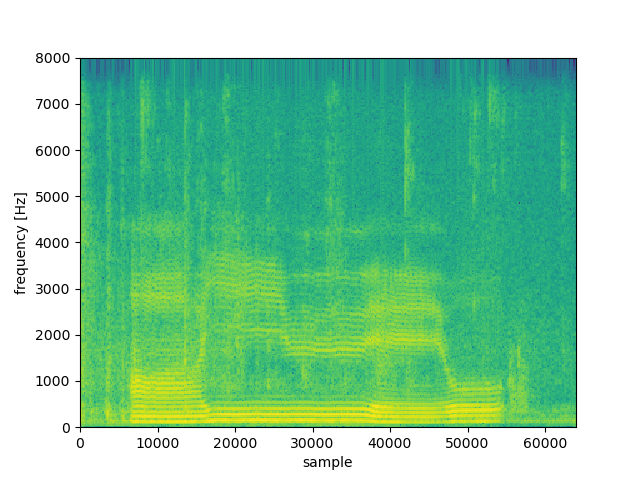
\includegraphics[scale=0.5]{../ex05/plot-spectrogram.png}
  \caption{「あいうえお」のスペクトログラム}
  \label{aiueo_spectrogram}
\end{figure}

ただし、利用した窓関数は長さが512, シフト長10msのハミング窓であり、スペクトログラムの縦軸は周波数、横軸は時間経過を表す。

\section{演習6 : np.fft.rfftとnp.fft.fftの違い}
$$
X_f = \frac{1}{\sqrt{N}} \sum_{t=0}^{N-1} x_t e^{-\frac{2\pi}{N}ift}  (f=0,...,N-1)
$$
$x_t (t=0,...,N-1)$が複素数であるとき、上式で定められる逆フーリエ変換を、高速フーリエ変換(FFT)に基づいて行うのがnp.fft.fftである。\par
ここで、$x_t$が実数の場合、$x_t e^{-\frac{2\pi}{N}ift}$ $(f=0,...,N-1)$の値は、$k$番目と$N-1-k$番目が複素共役になる。よって、$N$個のデータうち前半を計算できれば、後半は前半の複素共役として求められる。これを利用して計算回数を減らしたフーリエ変換の計算方法がnp.fft.rfftであり、実数値の信号$x_t$に対してはこれを利用することができる。

\end{document}